\section{Refactoring Patterns and Code smells}

By using the plugin \textit{SonarLint} in \textit{IntelliJ} I was able to find several code smells within the
scope of my chosen feature.

\subsection{JDisclosureToolBar class}


The \textit{JDisclosureToolBar} class, part of the JHotDraw project, exhibits several code smells.
These code smells potentially impact the maintainability, readability, and scalability of the code.
below is the code that is referred to in the code smell analysis table that is also below.

\begin{figure}[H]
    \centering
    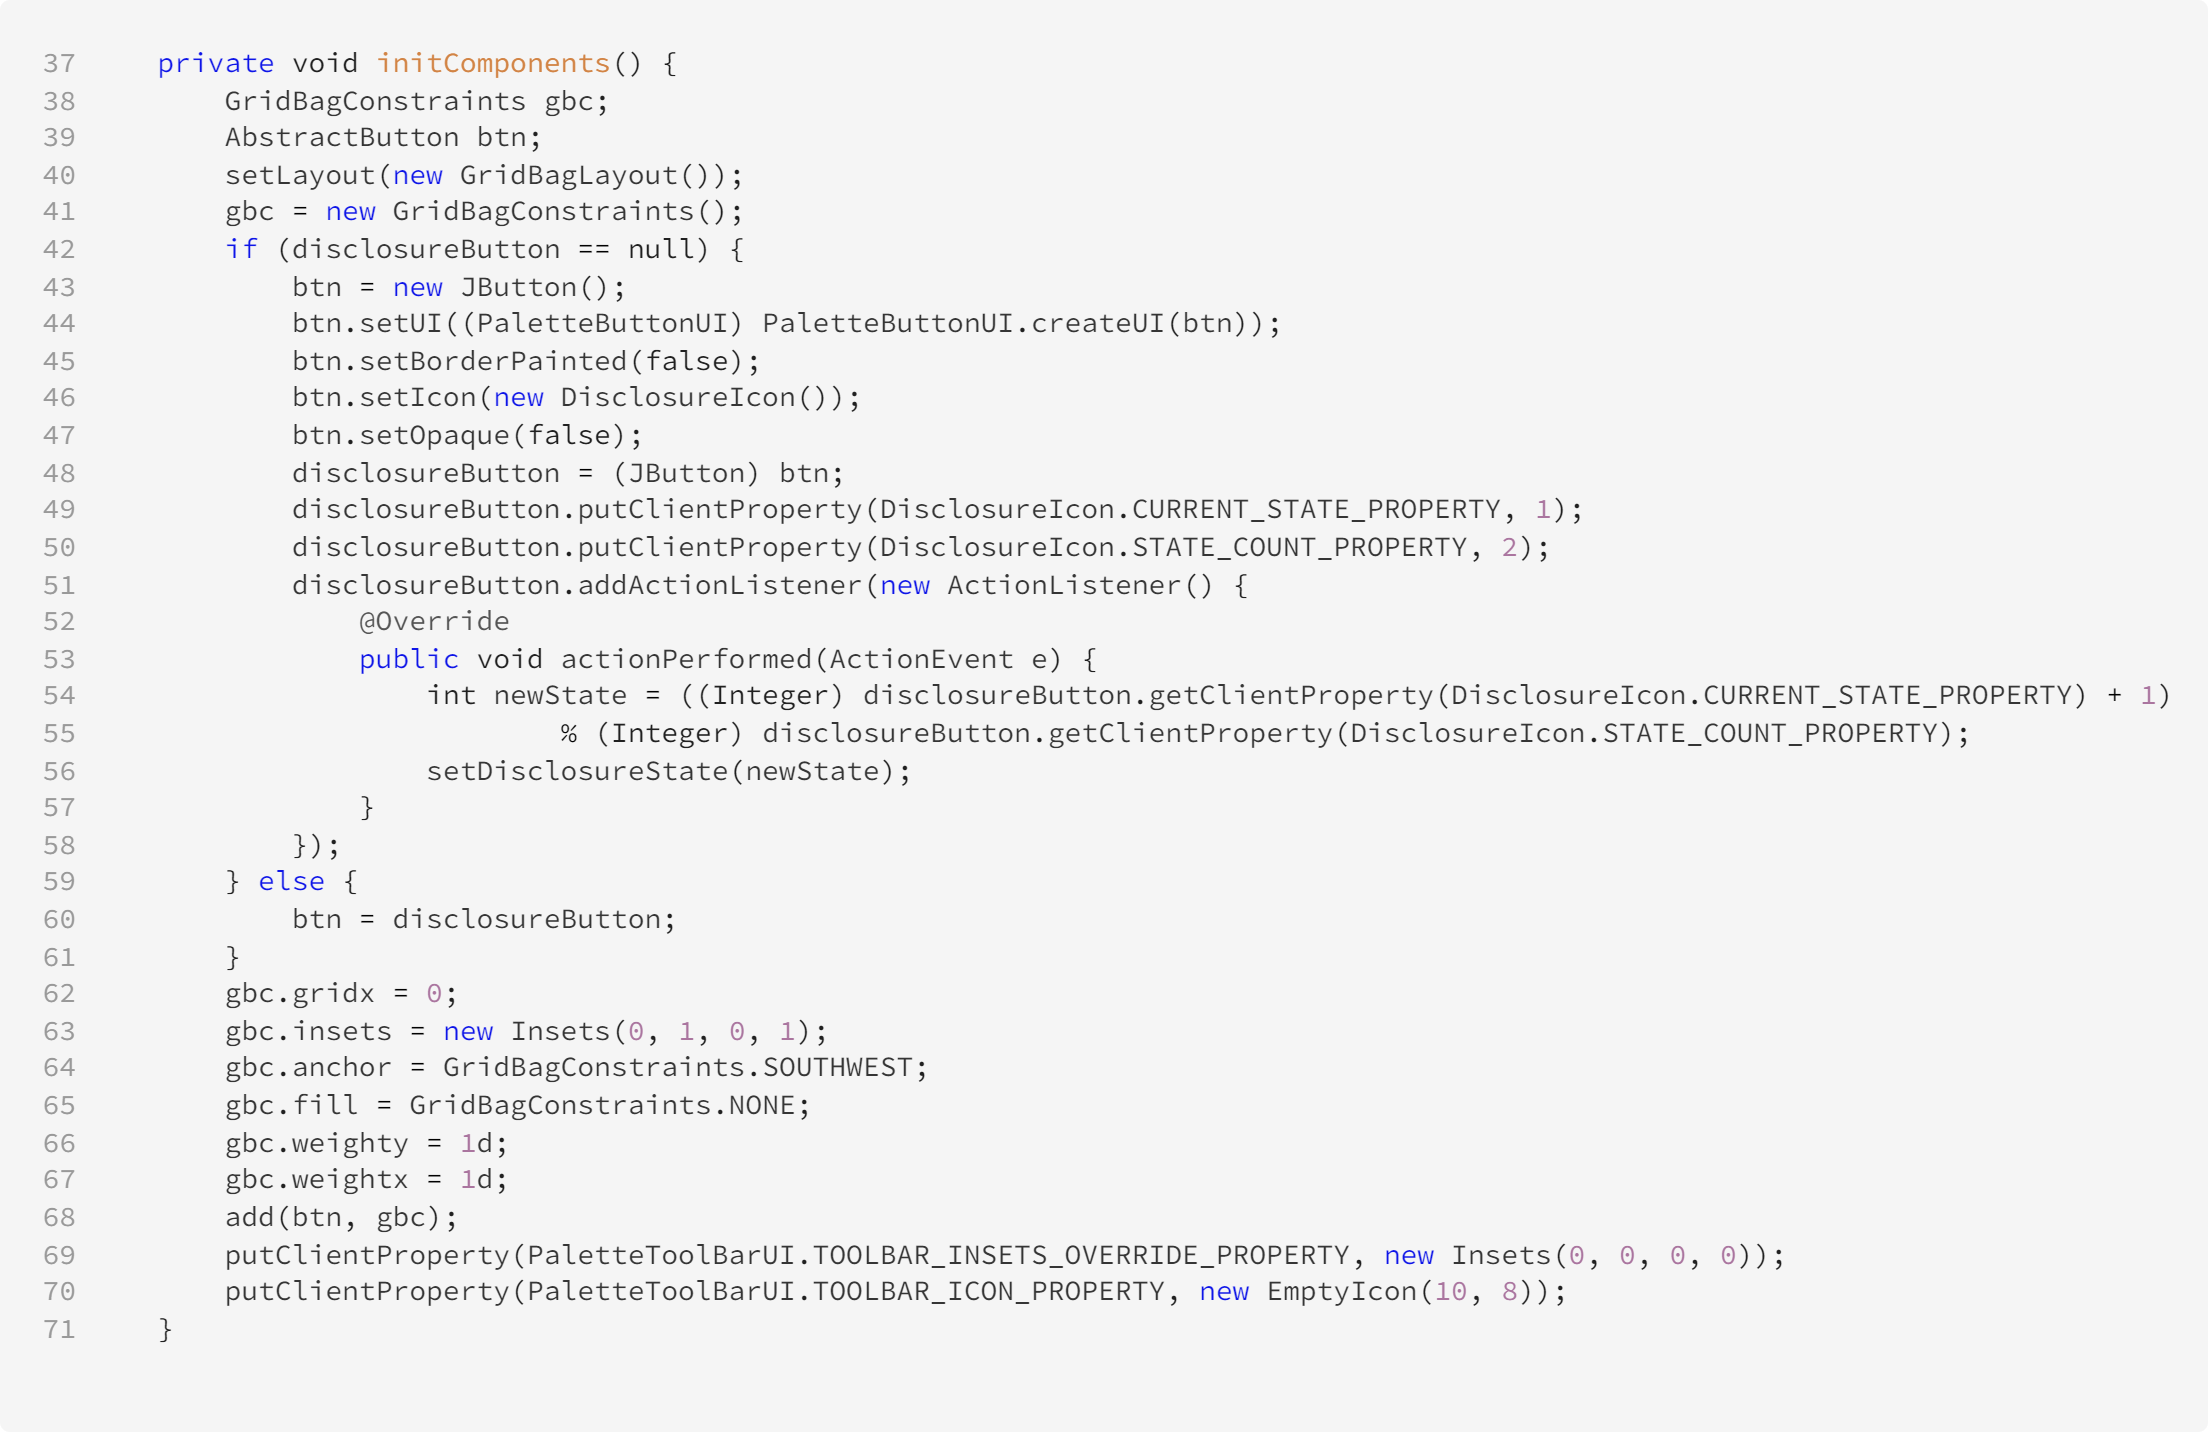
\includegraphics[width=\linewidth]{pic/initComponents.png}
    \caption{Orginal initComponents function}
    \label{fig:Orginal initComponents function}
\end{figure}


\begin{figure}[H]
    \centering
    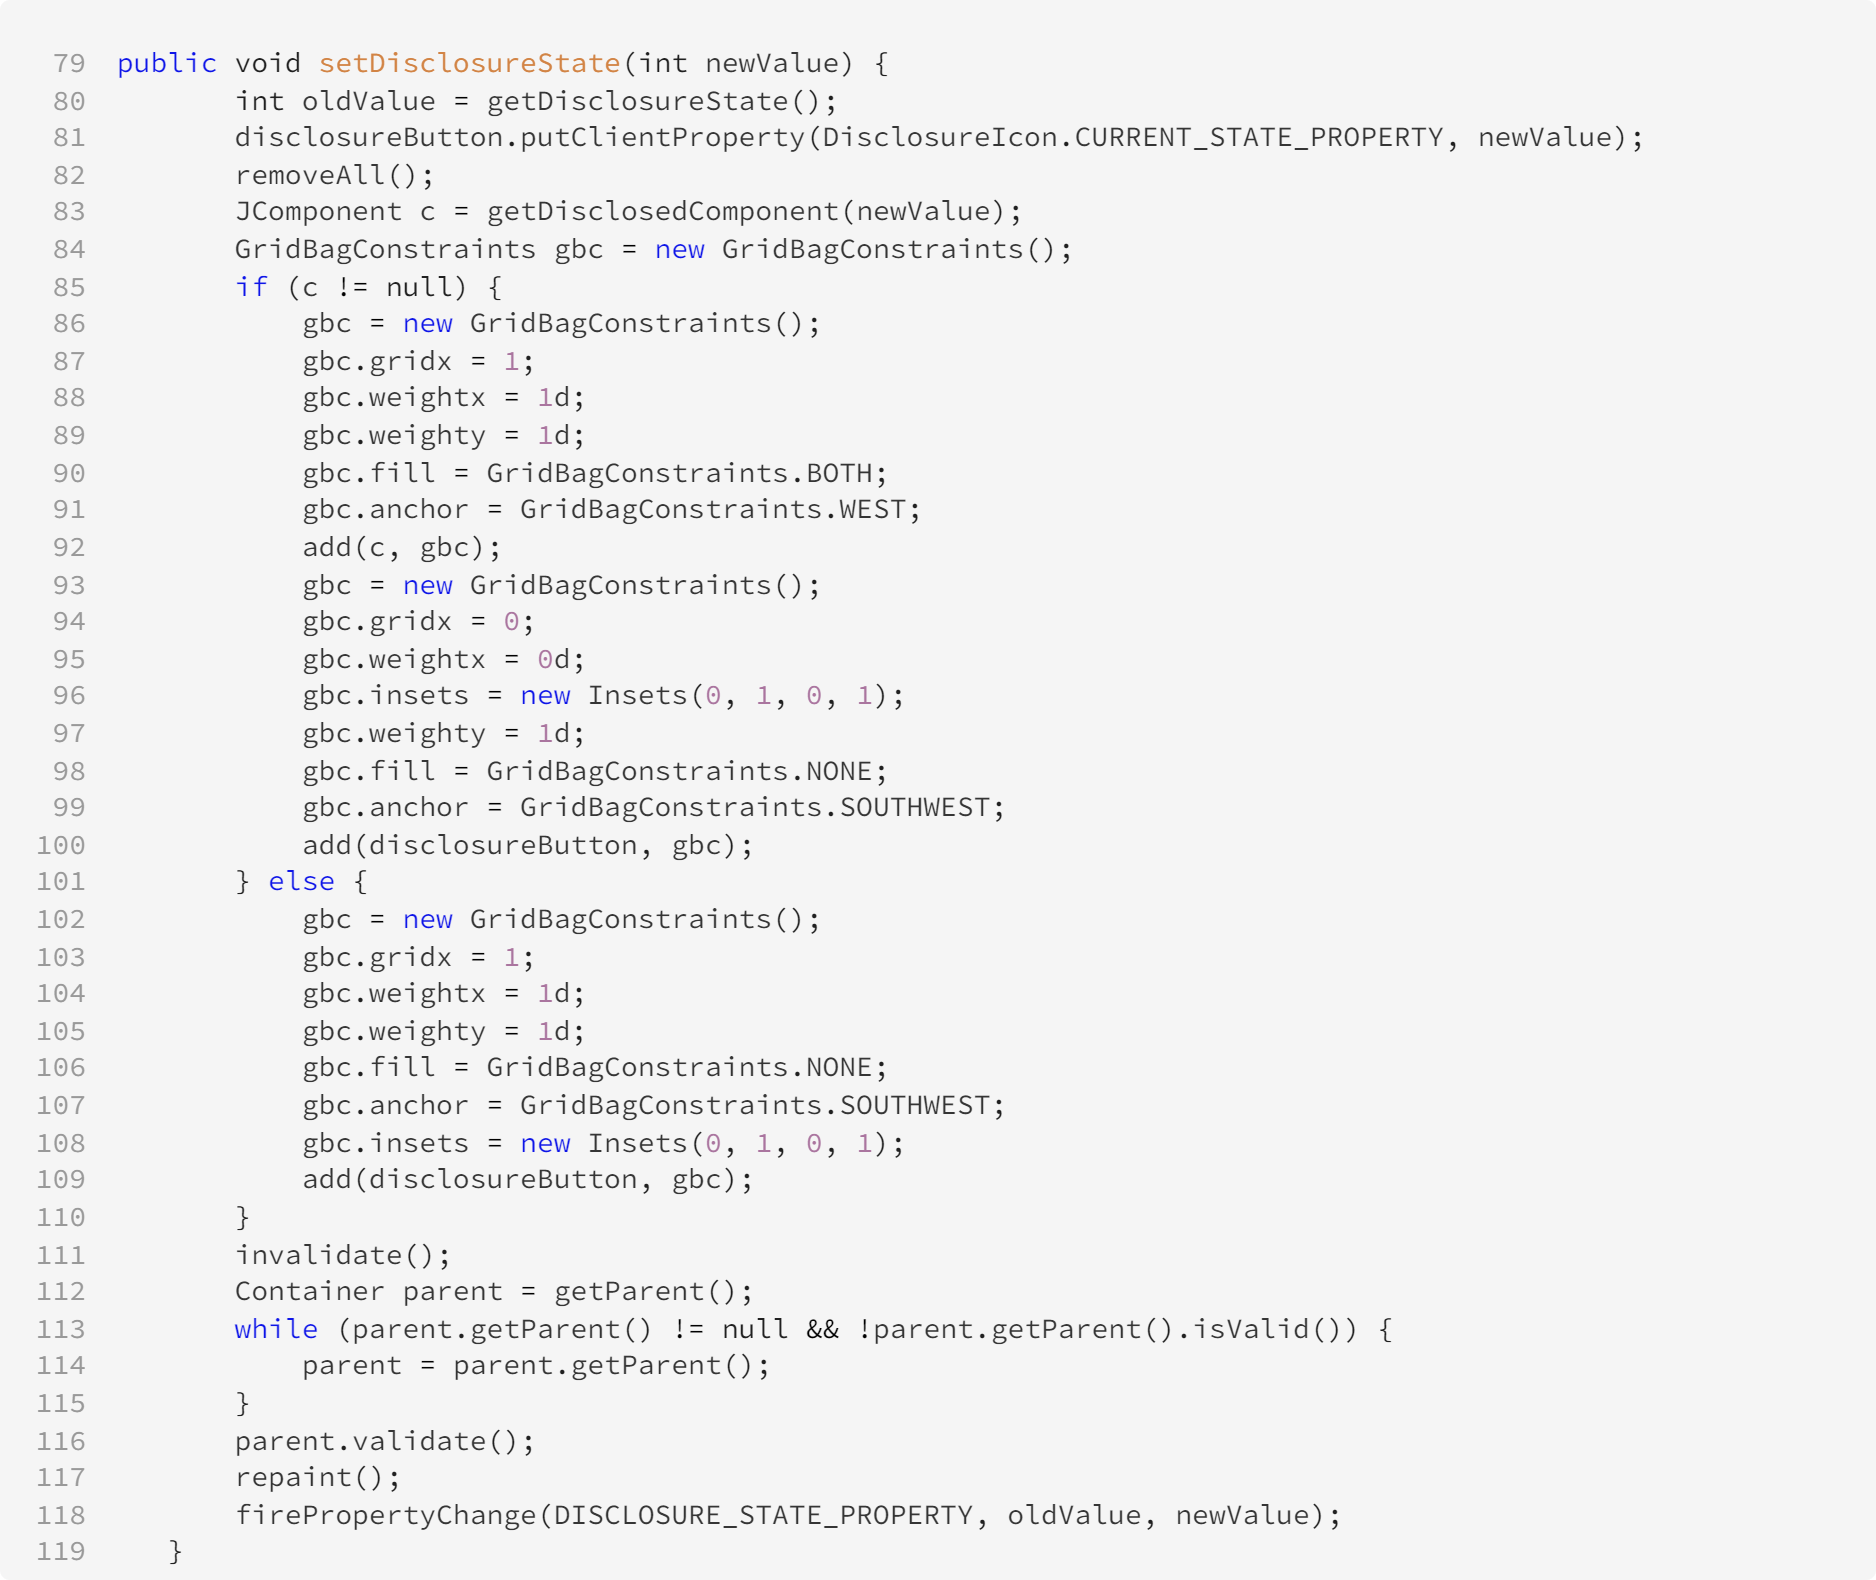
\includegraphics[width=\linewidth]{pic/setDisclosureState.png}
    \caption{Orginal setDisclosureState function}
    \label{fig:Orginal setDisclosureState function}
\end{figure}



\begin{table}[H]
    \centering
    \begin{tabular}{|l|p{6cm}|p{6cm}|}
        \hline
        \textbf{Method Name}        & \textbf{Description}                                                                                          & \textbf{Recommendation}                                        \\ \hline
        \textit{setDisclosureState} & \textit{setDisclosureState} is lengthy and handles multiple tasks, affecting readability and maintainability. & Break down into smaller, focused methods.                      \\ \hline
        \textit{setDisclosureState} & Repeated setup of \textit{GridBagConstraints} in multiple methods.                                            & Abstract common setup into a separate method or utility class. \\ \hline
        \textit{initComponents}     & \textit{initComponents} mixes UI element creation with layout management.                                     & Separate UI creation from layout management.                   \\ \hline
        \textit{initComponents}     & Unnecessary conditional logic in \textit{initComponents}.                                                     & Review the necessity and simplify if possible.                 \\ \hline
    \end{tabular}
    \caption{Code Smell Analysis for JDisclosureToolBar Class}
    \label{table:codesmell}
\end{table}

\subsection{PaletteToolbarUI class}


The \textit{PaletteToolbarUI} class in JHotDraw, designed for managing toolbars in a specific UI context, presents various code smells.
These issues potentially affect the code's maintainability, readability, and scalability.
The subsequent analysis and illustrations focus on specific methods within this class where these code smells are evident.
below is the code that is referred to in the code smell analysis table that is also below.

\begin{figure}[H]
    \centering
    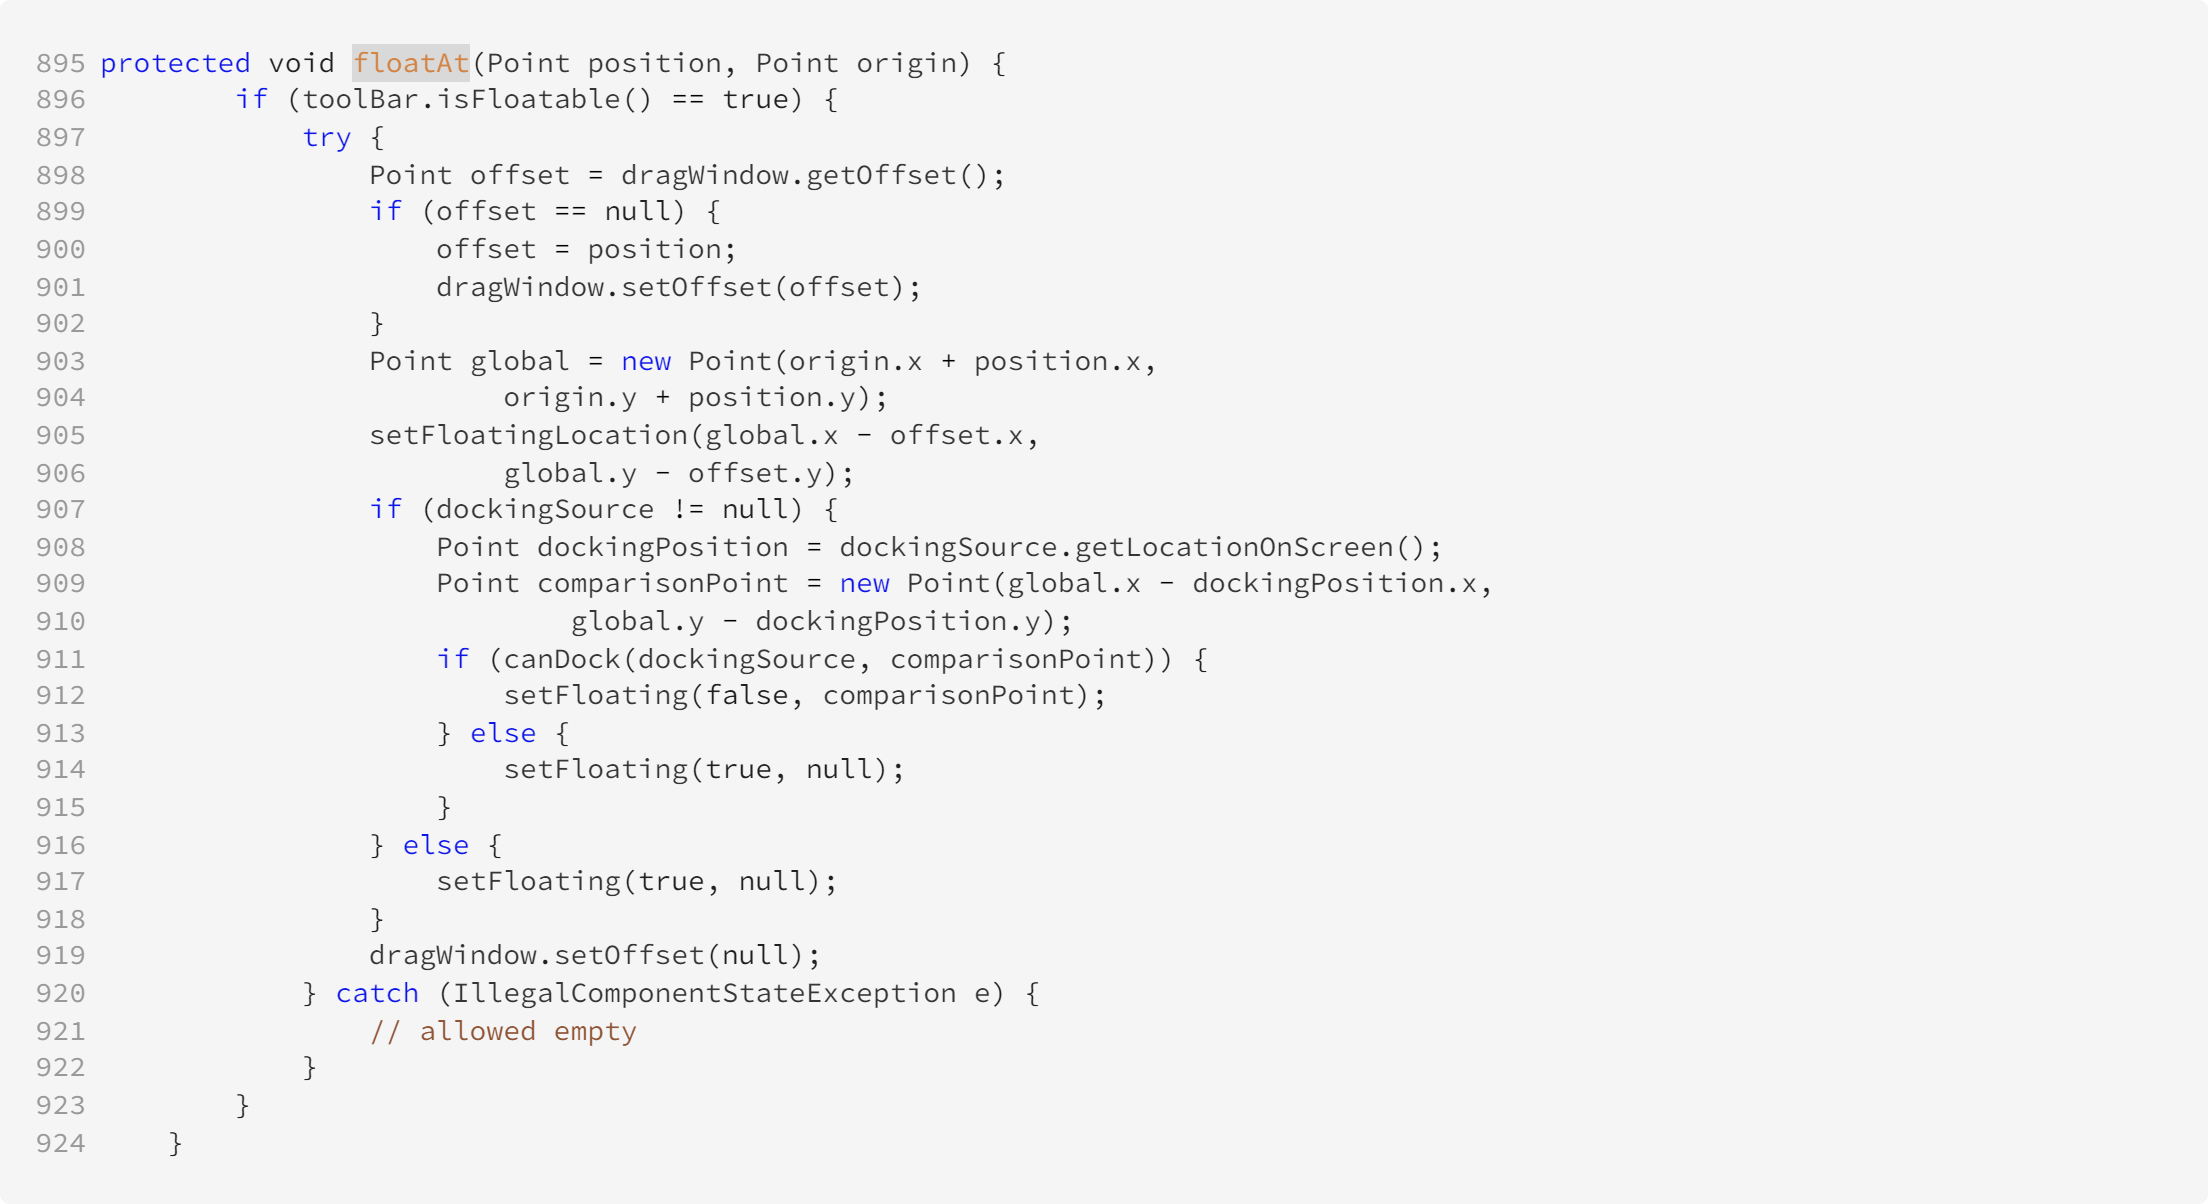
\includegraphics[width=\linewidth]{pic/floatAt.png}
    \caption{Orginal floatAt function}
    \label{fig:Orginal floatAt function}
\end{figure}


\begin{figure}[H]
    \centering
    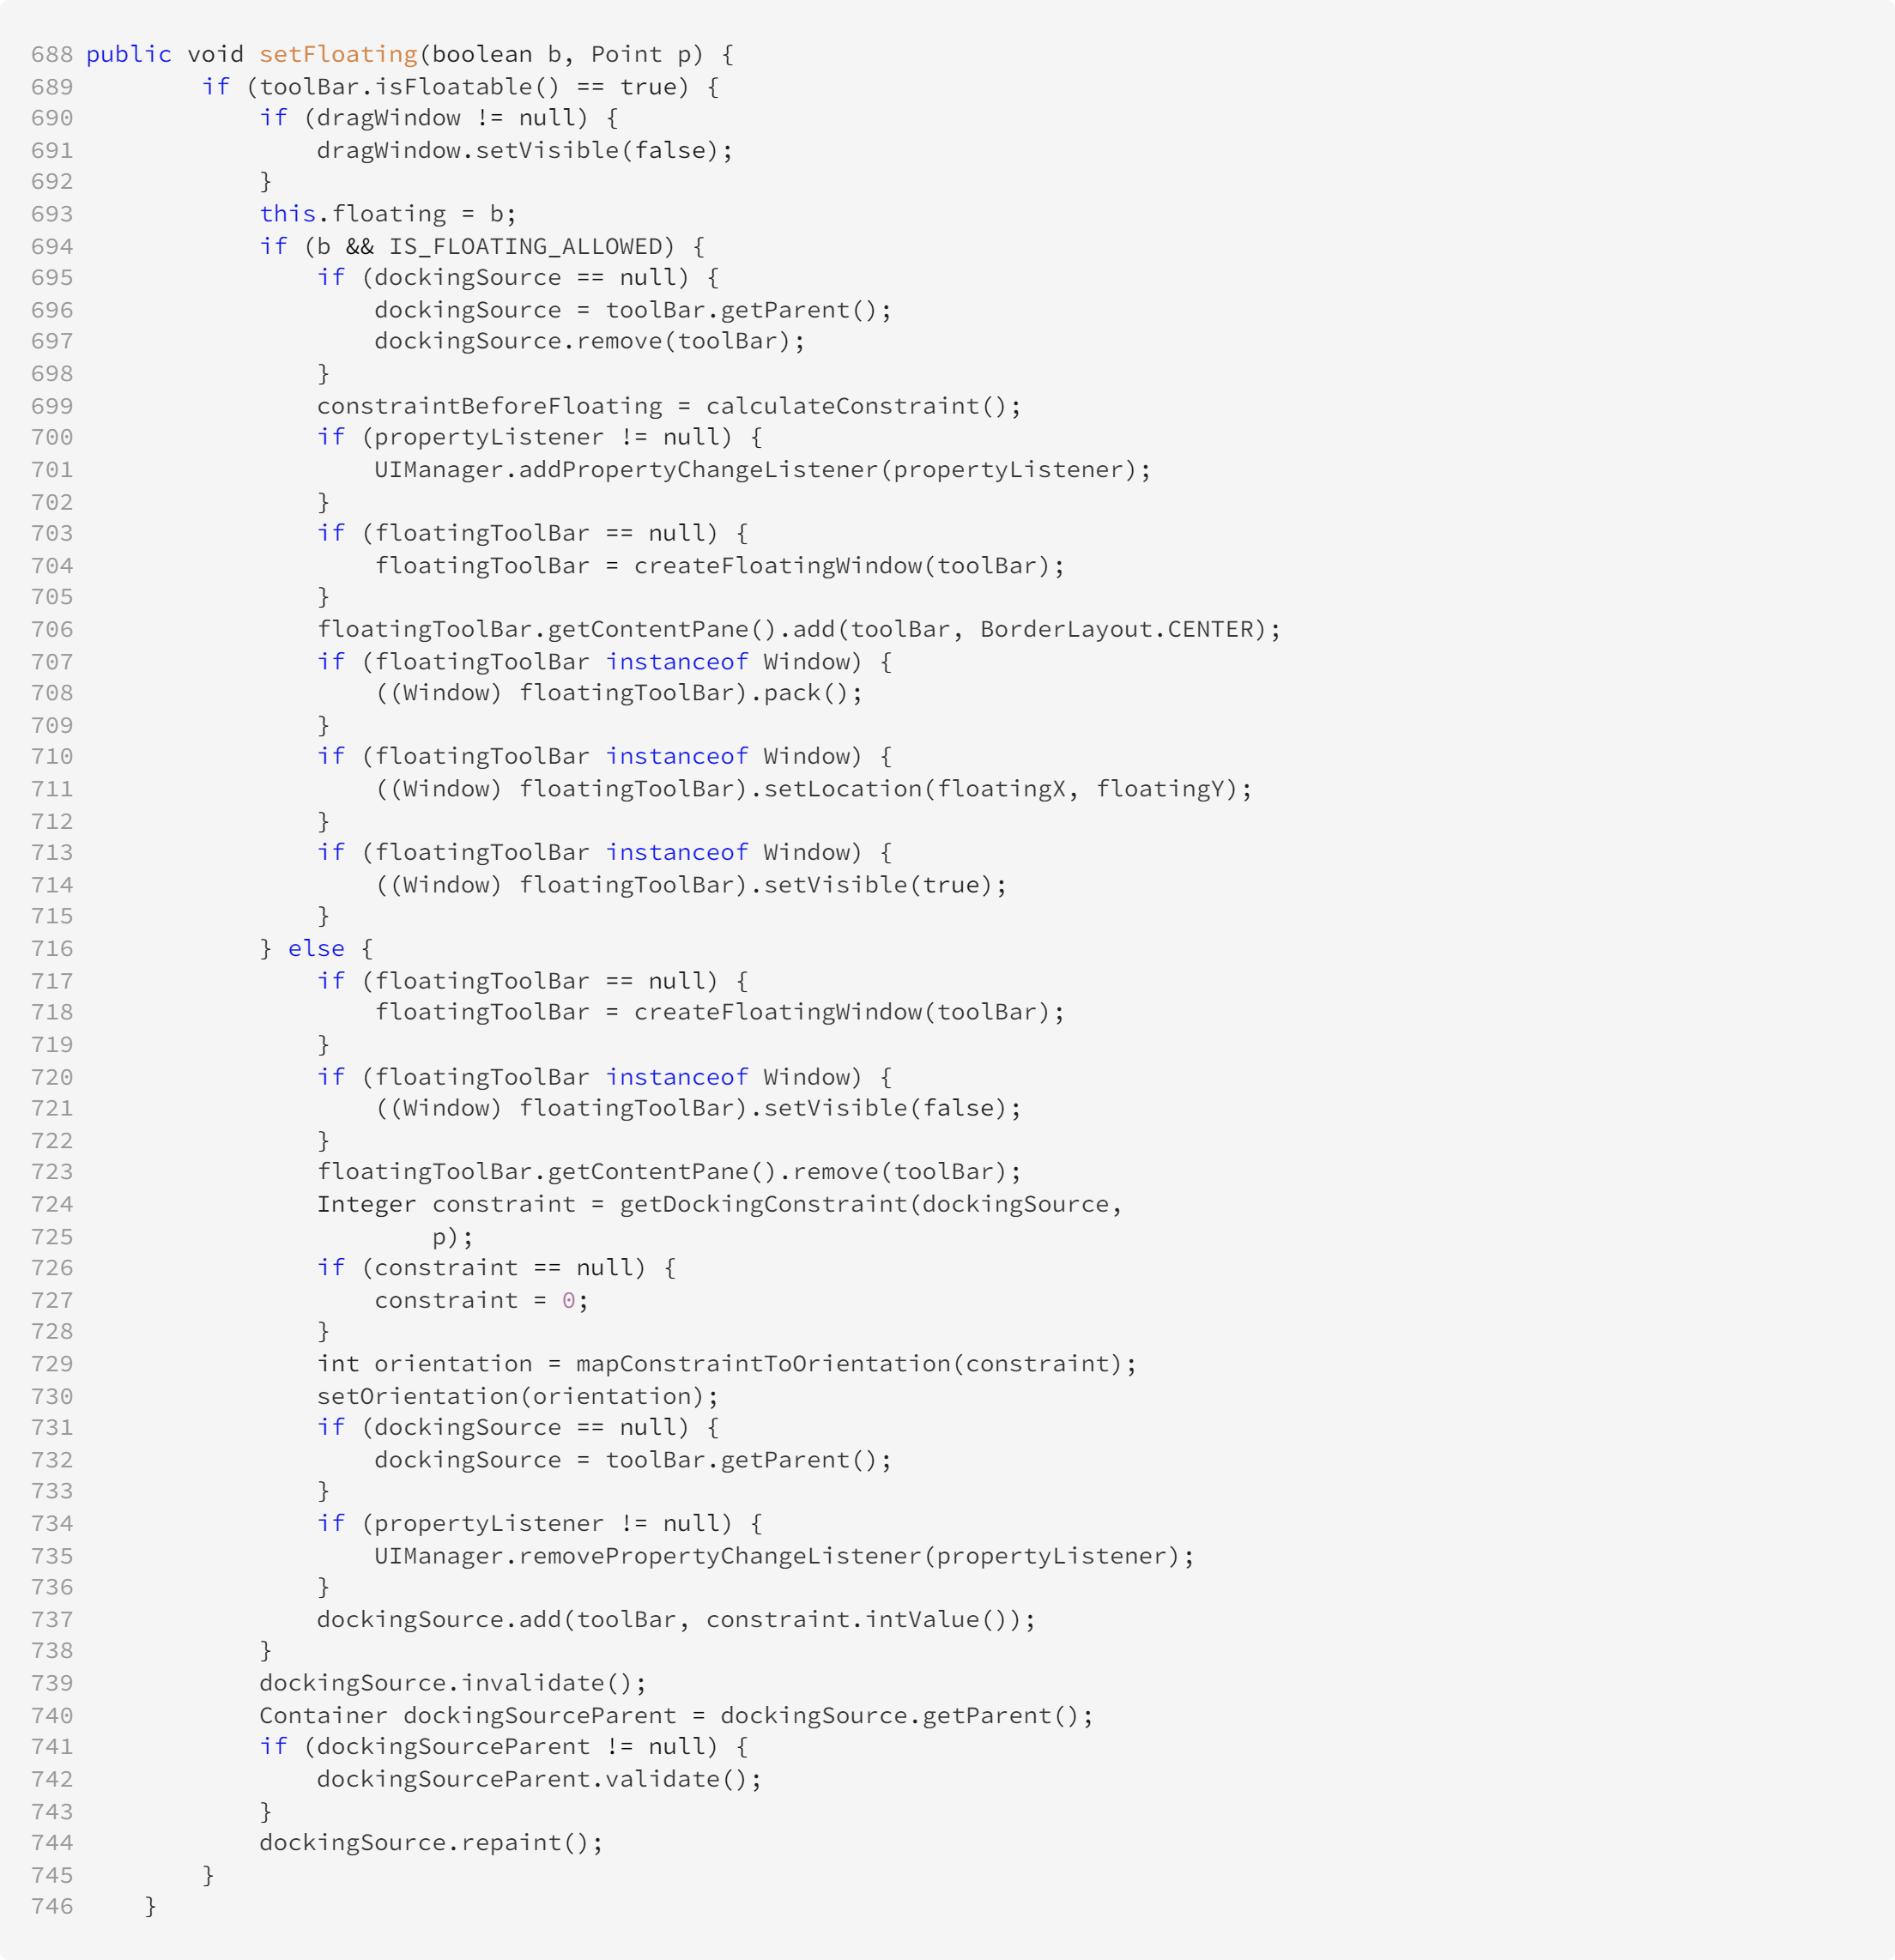
\includegraphics[width=\linewidth]{pic/setFloating.png}
    \caption{Orginal setFloating function}
    \label{fig:Orginal setFloating function}
\end{figure}

\begin{figure}[H]
    \centering
    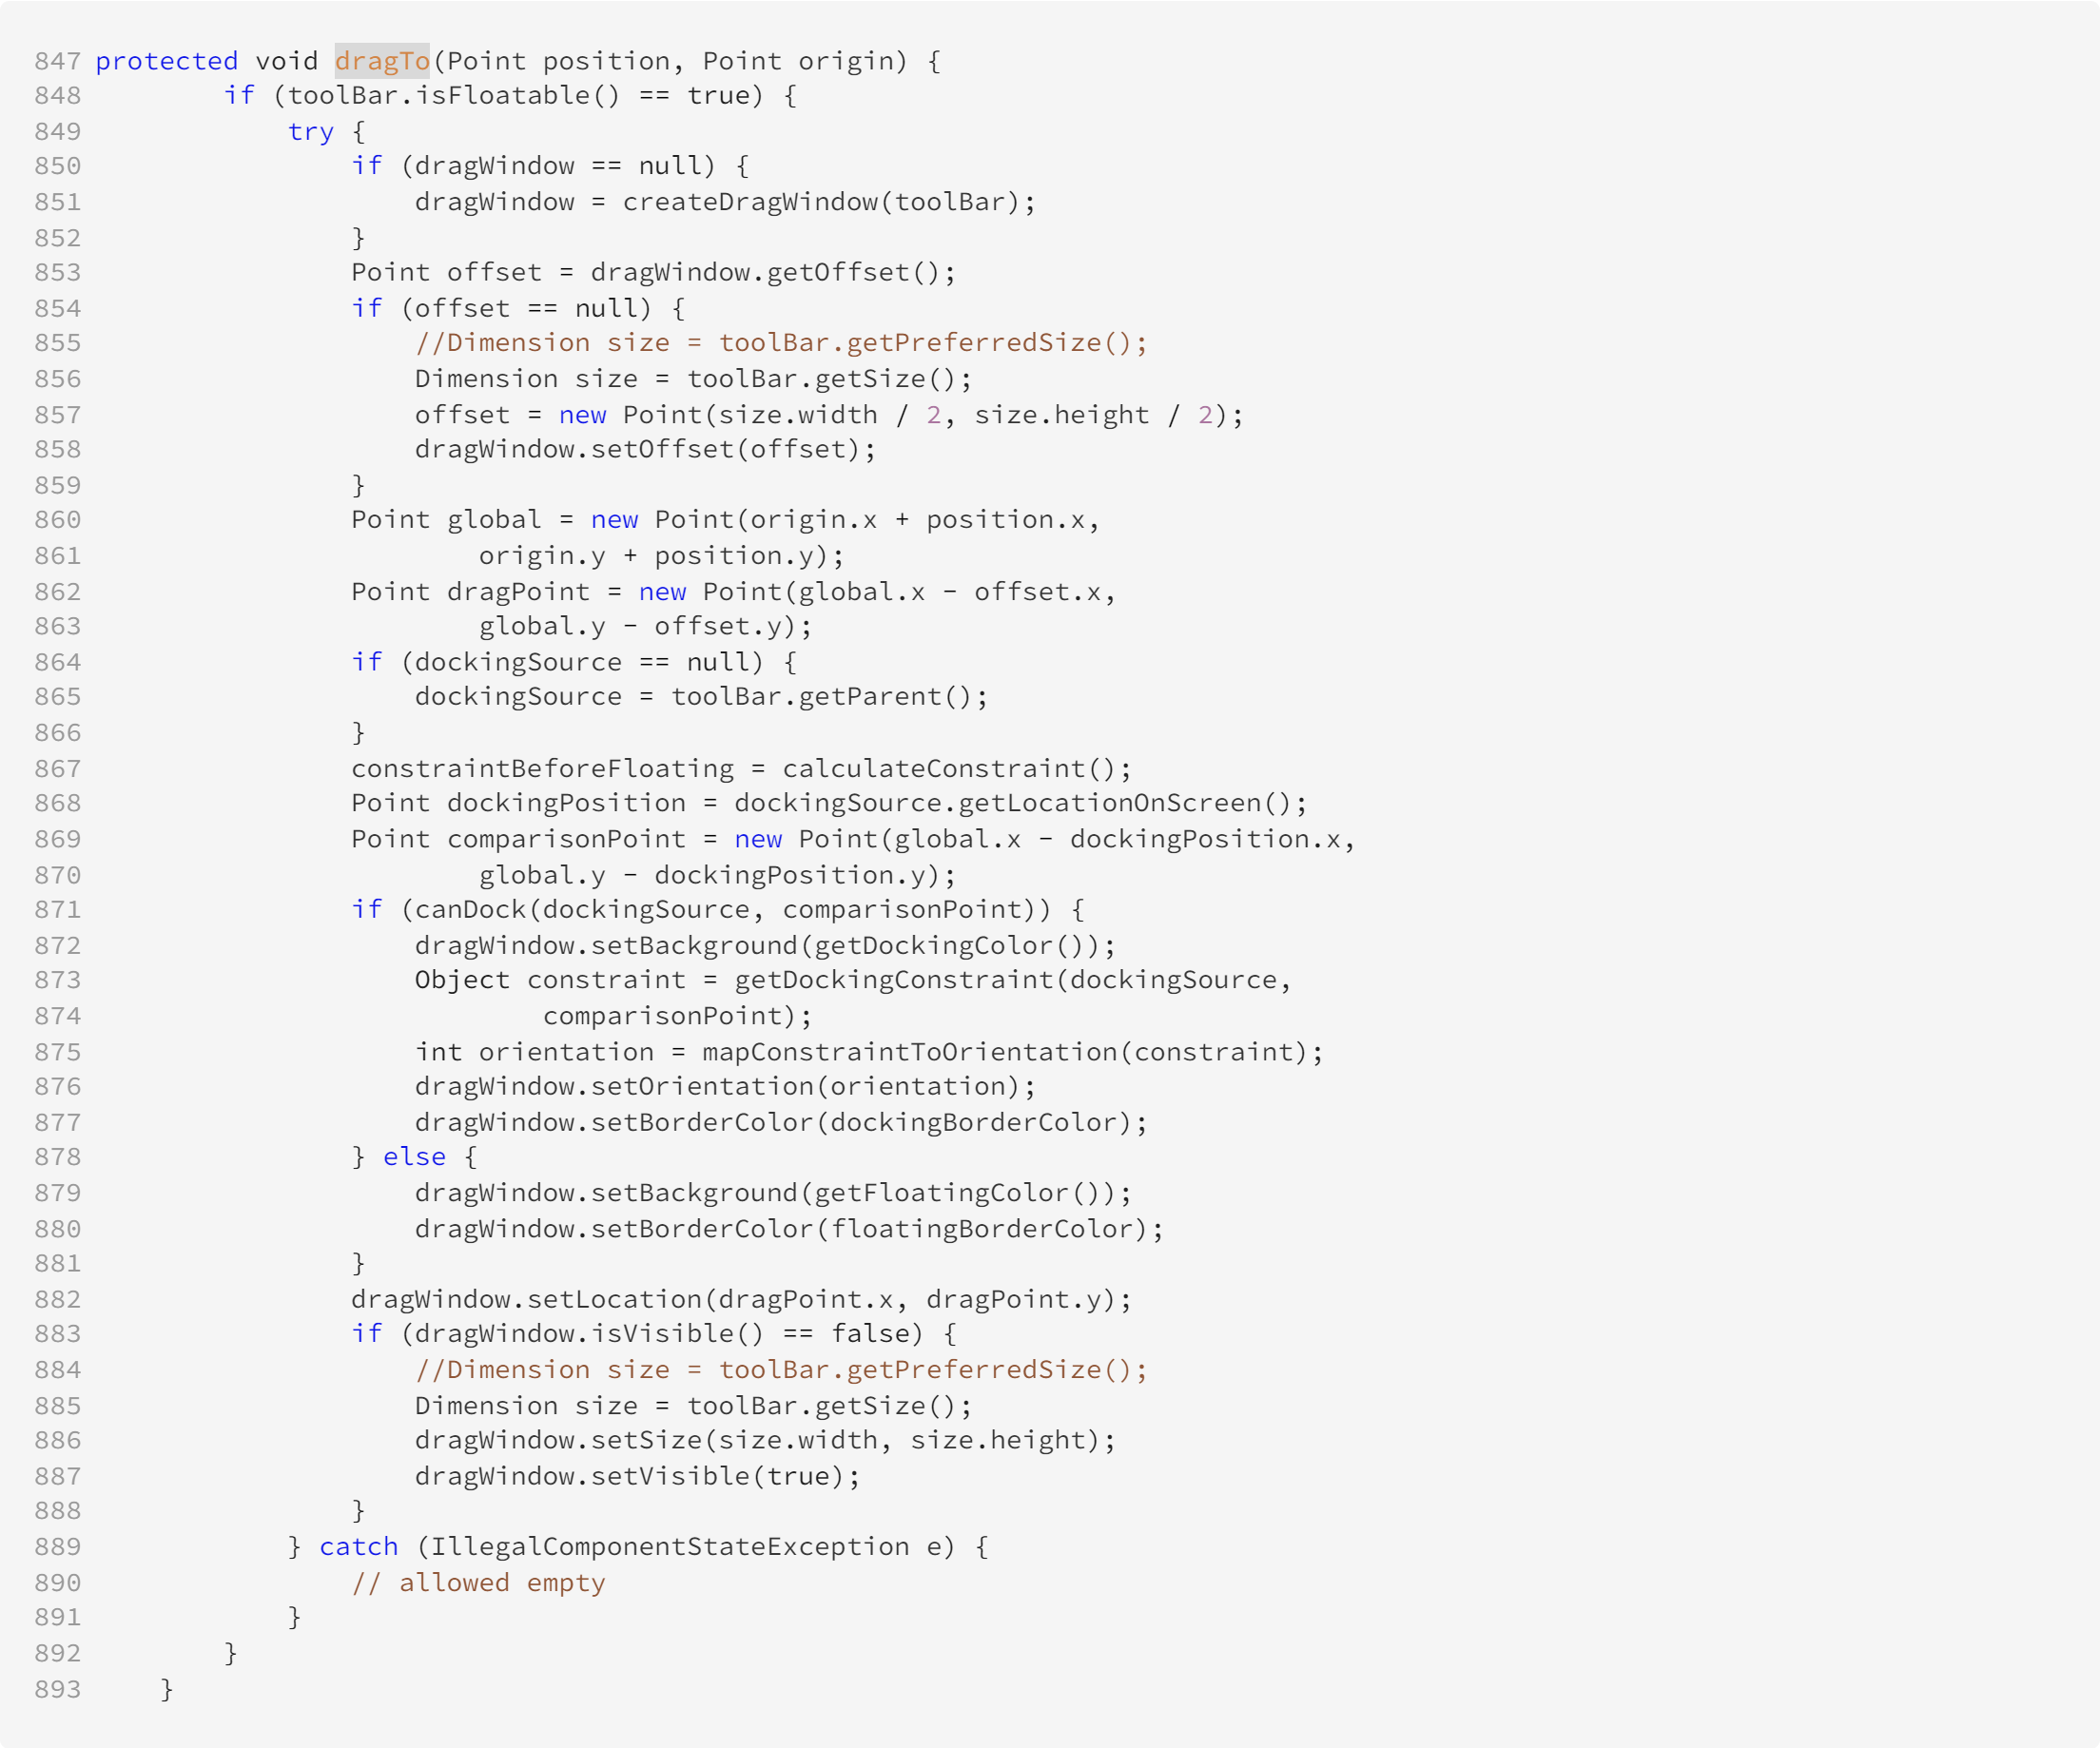
\includegraphics[width=\linewidth]{pic/dragTo.png}
    \caption{Orginal dragTo function}
    \label{fig:Orginal dragTo function}
\end{figure}


\begin{table}[H]
    \centering
    \begin{tabular}{|l|p{6cm}|p{6cm}|}
        \hline
        \textbf{Method Name} & \textbf{Description}                                                     & \textbf{Recommendation}                                                \\ \hline
        \textit{setFloating} & The method is doing too much, affecting readability and maintainability. & Break down into smaller, more focused methods.                         \\ \hline
        \textit{setFloating} & Multiple nested if-else statements increase complexity.                  & Refactor to reduce nested conditionals and simplify logic.             \\ \hline
        \textit{dragTo}      & The method is quite lengthy and performs many tasks.                     & Break down into smaller, more focused methods.                         \\ \hline
        \textit{dragTo}      & Use of similar calculations and procedures as seen in other methods.     & Abstract common functionality into a separate method or utility class. \\ \hline
        \textit{floatAt}     & The method is overly long.                                               & Break down into smaller, more focused methods.                         \\ \hline
        \textit{floatAt}     & Contains logic that appears to be duplicated from `dragTo`.              & Abstract common functionality into a separate method or utility class. \\ \hline
    \end{tabular}
    \caption{Code Smell Analysis for PaletteToolbarUI Class}
    \label{table:codesmell-palette}
\end{table}






